\makeatletter
\def\input@path{{styles/}}
\makeatother


\documentclass[12pt,a4paper]{article}
\usepackage{booktabs} 
\usepackage{multirow}
\usepackage[T1]{fontenc}
\usepackage[utf8]{inputenc}
\DeclareUnicodeCharacter{0301}{\'{e}}
\usepackage{hyperref}
\usepackage{xcolor}
\hypersetup{
  setpagesize  = false,
  colorlinks   = true,    % Colours links instead of ugly boxes
  urlcolor     = blue,    % Colour for external hyperlinks
  linkcolor    = black,   % Colour of internal links
  citecolor    = black    % Colour of citations
}
\urlstyle{same} 
\usepackage{authblk}
\usepackage{geometry}
\usepackage{setspace}
\usepackage{verbatim}
\usepackage{amsmath}
\usepackage{amssymb}
\usepackage{gensymb}
\usepackage{ragged2e} 
\usepackage{minted}
\usemintedstyle{tango}
\usepackage{amsfonts}
\usepackage{cancel}
%\usepackage{lineno}
\usepackage{tabularx}
\usepackage{lmodern}
\usepackage{fancyhdr}
\usepackage{float}
\usepackage{placeins}
\usepackage{graphicx}   % incluir imagens
\usepackage{subcaption} % subfiguras
\usepackage{seqsplit} 

\usepackage[backend=biber, style=ama]{biblatex}
\addbibresource{referencias.bib}


\setcounter{page}{1} % página inicial do artigo
%==========================================================================
% Margens e tamanho da página
%==========================================================================
\setlength{\paperwidth}{19cm}\setlength{\paperheight}{29cm}
\setlength{\textwidth}{16cm}\setlength{\textheight}{23cm}
\setlength{\oddsidemargin}{2cm}
\setlength{\headheight}{\baselineskip}
\setlength{\topmargin}{.2cm}
\setlength{\footskip}{1cm}\addtolength{\footskip}{.5\baselineskip}
\addtolength{\topmargin}{-1in}
\addtolength{\oddsidemargin}{-1.18in}
\setlength{\evensidemargin}{\oddsidemargin}
%==========================================================================
% Definições diversas
%==========================================================================
\setlength{\parindent}{1cm}
\newcommand{\abstractinenglishname}{Abstract}
\newcommand{\keywordsenglishname}{Keywords}

%==========================================================================
%Abstract (englishabstract)
%==========================================================================
\renewcommand{\abstractname}{Abstract}
\renewenvironment{abstract}{
        \begin{center}
	\begin{minipage}{14cm}
	{\textbf{\abstractname:}}
}{
        \end{minipage}
	\end{center}
}
%==========================================================================
% Palavras-chave (keywords) e Keywords (keywordsenglish)
%==========================================================================

\newenvironment{keywordsenglish}{
        \def\abstractname{\emph{\keywordsenglishname}}
	\begin{abstract}
}{
        \end{abstract}
}

%==========================================================================
% Artigo
%==========================================================================

\title{\textbf{Radiomics applied to skin lesion classification in HFUS images}}
\author[1]{Lucas Gambim Guedes\thanks{Corresponding author: Lucas Gambim Guedes\\Address: R. Sarmento Leite, nº 245 - Centro Historico, Porto Alegre, RS, Brazil.\\Phone: +55 (51) 99934-9634\\Email: \href{mailto:lucas.guedes@ufcspa.edu.br}{lucas.guedes@ufcspa.edu.br}}}
\author[1]{Isabela Rocha Veiga da Silva}
\author[1]{Thatiane Pianoschi}
\author[1]{Viviane Rodrigues Botelho}


\affil[1]{Federal University of Health Sciences of Porto Alegre, Porto Alegre, RS, Brazil}

\date{}
%==========================================================================
% Não editar o cabeçalho
%==========================================================================
\fancyhead[L]{\small Machine Learning skin lesion analysis in HFUS imaging, 2026 | Guedes \textit{et. al}
%| DOI: https://doi.org/xxxxx \newline Licença Creative Commons CC BY-ND 4.0
}
%==========================================================================
% Não editar o cabeçalho
%==========================================================================
\fancyhead[R]{\thepage}
\pagestyle{fancy}
\linenumbers

\begin{document}

\maketitle

\vspace{-1em}
\begin{center}
\textbf{Machine Learning skin lesion analysis in HFUS imaging} \\
\textbf{Manuscript Category:} Original Article
\end{center}
\vspace{0.4cm}

\begin{abstract}

This study evaluates the performance of classical machine learning classifiers trained with radiomic features extracted from high-resolution ultrasound images (HFUS), a non-invasive diagnostic modality that provides high-resolutions images from the epidermis to the deep fascia, to classify cutaneous lesions according to their malignancy. First-order and texture features were extracted, with selection performed via ANOVA F-score and Mutual Information, and 23 classifiers were evaluated in three datasets (BW-mode, Doppler and combined). The best model, a Gaussian SVM, achieved an accuracy of $95.0\%$, sensitivity of $100\%$, AUC of 0.978 and a performance equivalent to deep learning architectures reported in the literature. The results indicate that radiomics features capture sufficient textural and morphological information to match the performance of dedicated CNNs, with the advantage of lower computational cost and greater interpretability. 

% tornando essa abordagem especialmente adequada a cenários clínicos com recursos e dados limitados 

\end{abstract}

\begin{keywordsenglish}
HFUS, Machine learning classifiers, skin neoplasms, ultrasonography, texture analysis
\end{keywordsenglish}


\doublespacing

\section{Introduction}

Skin cancer is is the most frequently diagnosed neoplasm in the world, the most common in Western populations and also most complex in humans \cite{Juan2023, Zhu2024}. However, when detected in early stages the overall survival rate can reach $99\%$. This effectiveness decreases as the disease progresses, since the rate drops when the disease spreads beyond the skin \cite{GOYAL2020}. To make this possible, dermatologists evaluate lesions through different analysis methods and imaging techniques. Among available non-invasive methods are dermoscopy, the confocal microscopy and other medical imaging modalities; however, these techniques still present limitations in obtaining information about the depth of the lesion \cite{Xiao2025, Zhu2024}. High-frequency ultrasound helps overcome this limitation by providing high-resolution images from the epidermis to deep fascia, showing potential for differentiating benign and malignant skin lesions \cite{daSilva2026, Czajkowska2021}.

Although, these techniques provide detailed morphological information about skin lesions, the analysis process is still fundamentally based on the specialist's experience and perception \cite{Qin2025}. This makes the diagnose susceptible to subjectivities that can result in interpretative errors and delays in reaching a diagnostic conclusion \cite{Qin2025}. Furthermore, if the non-invasive evaluation is classified as inconclusive, confirmation depends on histopathological exam, which is surgical and painful \cite{Qin2025, Zhu2024}.

Given this scenario, Machine Learning (ML) and Deep Learning (DL) techniques have emerged as promising tools to assist medical image diagnosis \cite{daSilva2026}. Algorithms based on convolutional neural networks have been widely applied to various medical images modalities, demonstrating performance comparable to human specialists in classification and detection tasks \cite{LaverdeSaad2021}. In the dermatologic ultrasound context, recent studies show growing interest in this approach Laverde-Saad et al. (2022) trained a pre-build CNN (EfficientNet B4) to distinguish benign and malignant lesions in HFUS images, achieving an accuracy of $77.1\%$ \cite{LaverdeSaad2021}. Silva et al. (2026), in work previously developed by our research group, advanced this direction by combining BW-mode and Doppler images in four multimodal CNN architectures. Of these, the HFUS-Doppler model achieved the best performance, reaching an accuracy of up to $95\%$ and an AUC of 0.98 \cite{daSilva2026}. Despite these promising results, deep learning models present a relevant limitation for clinical application: their predictions are often difficult to interpret, since the feature extraction process occurs implicitly within the neural network \cite{Qin2025}. Furthmore, effictive neural network training requires a hing computational and data cost \cite{LaverdeSaad2021}. 

In this context, radiomics emerge as a extraction process of a large number of features related to morphological and textural information from medical images, making quantitative information about lesions accessible that is not perceptible through direct visual assessment \cite{Lambin2017}. These extracted characteristics, which include intensity, shape, texture, and wavelet transform values, capture characteristics of the lesion's phenotype that are distinct from or complementary to information obtained by other methods \cite{Lambin2017}.

Despite growing interest in the application of radiomics to medical images, few studies have extracted these features from ultrasound images to classify skin tumors with machine learning classifiers \cite{Qin2025}. Most existing studies focus on the use of DL \cite{Surkov2024, Bibi2026, Czajkowska2021-2}. This gap represents an opportunity to evaluate which radiomic features are most discriminative for this classification task.

Given this, the present work aims to evaluate the performance of several classical machine learning classifiers trained with radiomic features extracted from HFUS images to assess the malignancy of cutaneous lesions, comparing the results obtained with those reported by Silva et al. (2026). 

\section{Materials and Methods}

The methodological workflow is organized into five main stages: (A) dataset and partitioning; (B) radiomic feature extraction; (C) feature selection; (D) Experimental Design and Cross-Validation; and (E) performance analysis.

\subsection{Dataset}

The dataset produced by Alfageme. \cite{BANCO2022} was used. It is composed of high-frequency ultrasound (HFUS) images in png format with a resolution of 240x240 pixels, acquired in BW and Doppler modes, shown in figure \ref{fig:datasetimg}, of cutaneous lesions accompanied by metadata available in the repository in csv format. The lesions are labeled into two categories for the binary classification task: benign and malignant, with a distribution of approximately $65.7\%$ and $34.3\%$ respectively \cite{daSilva2026}.

\begin{figure}[h]
    \centering
    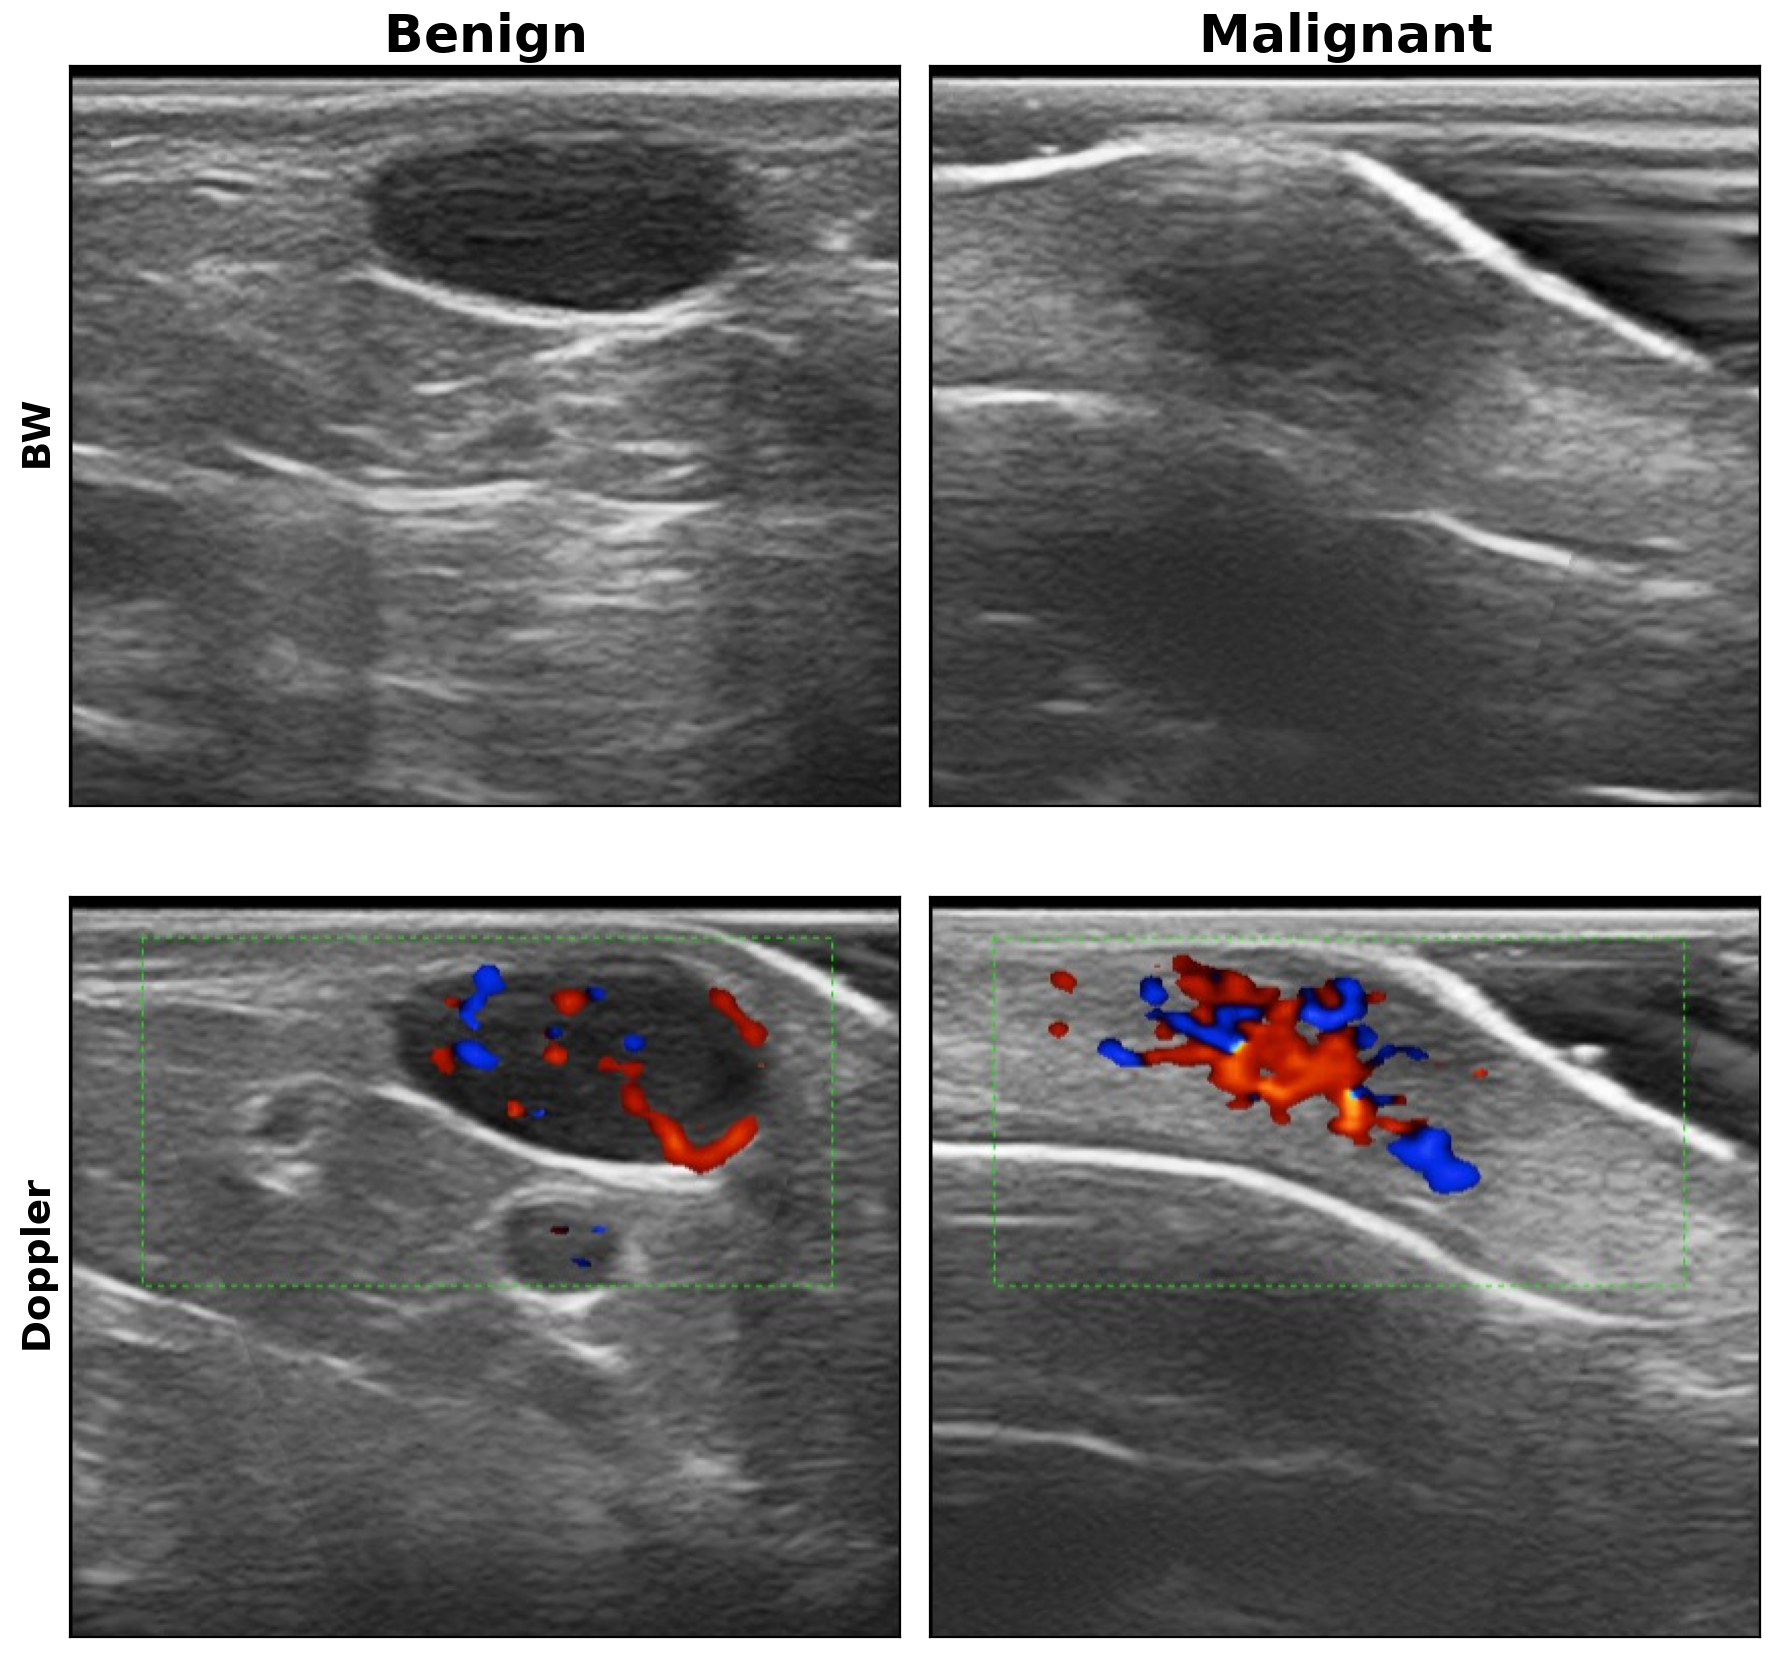
\includegraphics[width=0.7\textwidth]{Images/figure1_dataset_examples.png}
    \caption{Example HFUS images from the dataset, acquired in BW-mode (BW) and Doppler mode.}
    \label{fig:datasetimg}
\end{figure}

The images were stratified and split into two mutually exclusive subsets, so the split was as follows: $70\%$ allocated to train and $30\%$ to test. Stratification was adopted to preserve the original class proportion in both subsets, mitigating bias arising from imbalance between malignant and benign classes. 

Silva et al. (2026) documented inconsistencies in the dataset \cite{daSilva2026}. Corrected prior to feature extraction. Three procedures were carried out: (1) name correction of images at pitions 57, 59, and 90 in the metadata table, which had inverted acquisition modes; (2) standardization of file name formatting for images 32, 106, 107, and 137; and (3) exclusion of the records for images 6, 62, 74, and 121, where two images associated with the Doppler mode had been acquired, maintaining the same composition as Silva et al. (2026), in order to ensure direct comparability of the results \cite{daSilva2026}. 

\subsection{Radiomic Features Extraction}

Radiomic features were extracted from the HFUS images using the PyRadiomics library (version 3.1.0, Python 3.7), available for the Python language, for the extraction of quantitative features from medical images. Data processing and analysis were performed using Python 3.11, along with the following libraries: NumPy 1.26.4, pandas 2.2.3, Matplotlib 3.8.4, scikit-learn 1.5.2, Seaborn 0.13.2, and Pillow 12.2.0. For each image, 465 features were extracted, organized into the following main categories: first-order and texture features.

The first-order features (First-Order Statistics) describe the pixel intensity distribution (mean, variance, kurtosis, entropy), and the texture information is derived from co-occurrence and spatial dependence matrices as Gray Level Co-occurrence Matrix, Gray Level Run Length Matrix, Gray Level Size Zone Matrix, Gray Level Dependence Matrix and  Neighboring Gray Tone Difference Matrix (GLCM, GLRLM, GLSZM, GLDM, and NGTDM). All extracted features were calculated both on the original image and on the four sub-bands of the 2D wavelet decomposition (LL, LH, HL, and HH), where each of these is a decomposition of the original image in which a low-pass filter (L) and/or a high-pass filter (H) is applied separately in both the horizontal and vertical directions, in order to capture where in space certain frequencies (LL = general approximation; LH = horizontal edges; HL = vertical edges; HH = diagonal edges) occur. Extracting radiomic features from these sub-bands allows capturing local texture and morphology information of the lesions, which is suppressed by the frequency mixing in the original image.

Finally, 3 datasets were created with the extracted features: BW, containing only the information from BW-mode images; Doppler, which comprised only the characteristics of Doppler images; and the combined BW+Doppler, whose feature vector totaled 931 features per image.

\subsection{Feature Selection}

Given the high number of features, an exploratory step was conducted to analyze the relevance of each feature on the training set using SelectKBest from the ScikitLearn library, in order to rank the features.

Two statistical criteria were applied: the ANOVA F-score to assess the ratio of inter-class to inter-class variance, and Mutual Information to capture non-linear dependencies between each feature and the target label. To avoid information leakage (data leakage) from the test set, both scores were calculated exclusively on the training set.

\subsection{Experimental Design and Cross-Validation}

The feature relevance analysis motivated two parallel experimental scenarios, referred to as Track A and Track B, whose objective was to evaluate the impact of feature selection on classifier performance. In both tracks, the same 23 classifiers were applied to the same three datasets (BW, Doppler, BW+Doppler), keeping all other experimental conditions equal, with the only variable differing between tracks being the number of features used in training.

In Track A, the training pipeline consisted of three sequential steps: feature standardization via StandardScaler, selection of the K most discriminative features by SelectKBest with the ANOVA F-score criterion, and classifier training. In Track B, the data were standardized, the same criterion was applied, and the features were used in their entirety. Standardization, with StandardScaler, preceded the application of SelectKBest because the F-score was sensitive to variable scale; without it, features with larger magnitude could have been artificially favored. To determine the value of K in Track A, the pipeline was run for K = 5, 10, 15, 20, 30, 50, and 100.
The performance of each configuration (classifier x dataset) was estimated by cross-validation using the stratified 5-fold k-fold technique applied to the training set. In Track A, the feature selection step was performed within each fold, fitted exclusively on that fold's training data (such that the subset of K selected features could vary between folds), avoiding information leakage between training and validation.

At the end of cross-validation, the classifier with the highest mean AUC across folds was selected as the representative model for each track and dataset. This model was then retrained on the full training set and evaluated once on the test set, which remained isolated throughout the entire development process.

\subsection{Performance Analysis}

The final evaluation of each model was performed a single time on the test set, after retraining on the full training dataset. Performance was analyzed from two different decision threshold perspectives: first, using a threshold of 0.5, and second, using the threshold determined by the Youden index, present in the equation \eqref{youden-eq}, calculated on the internal validation subset of the training data.

For each threshold, the following metrics were calculated from the confusion matrix and the ROC curve: AUC, accuracy, sensitivity, specificity, and F1-score. AUC was chosen as the primary metric for comparison between models and tracks, since it is independent of the decision threshold. Sensitivity and specificity were reported separately given the clinical context of the problem, where sensitivity holds greater relevance in medical diagnoses.

\begin{equation}
    J = \text{Sensitivity} + \text{Specificity} - 1
    \label{youden-eq}
\end{equation}

\section{Results}
\subsection{Feature Analysis}

Table \ref{tab:kbest-ranking} presents the five most discriminative features per dataset and per criterion. In both tests and across all datasets, a predominance of features extracted from the wavelet decomposition sub-bands (especially LH and LL) is observed over the features extracted from the original image, which reinforces the decision to include the wavelet bands in the feature vector. However, the two criteria mostly select distinct sets of features: while the ANOVA F-score tends to highlight first-order entropy and uniformity features and GLCM/GLRLM, Mutual Information favors zone size dependence features (GLDM/GLSZM).

\begin{figure}[h]
    \centering
    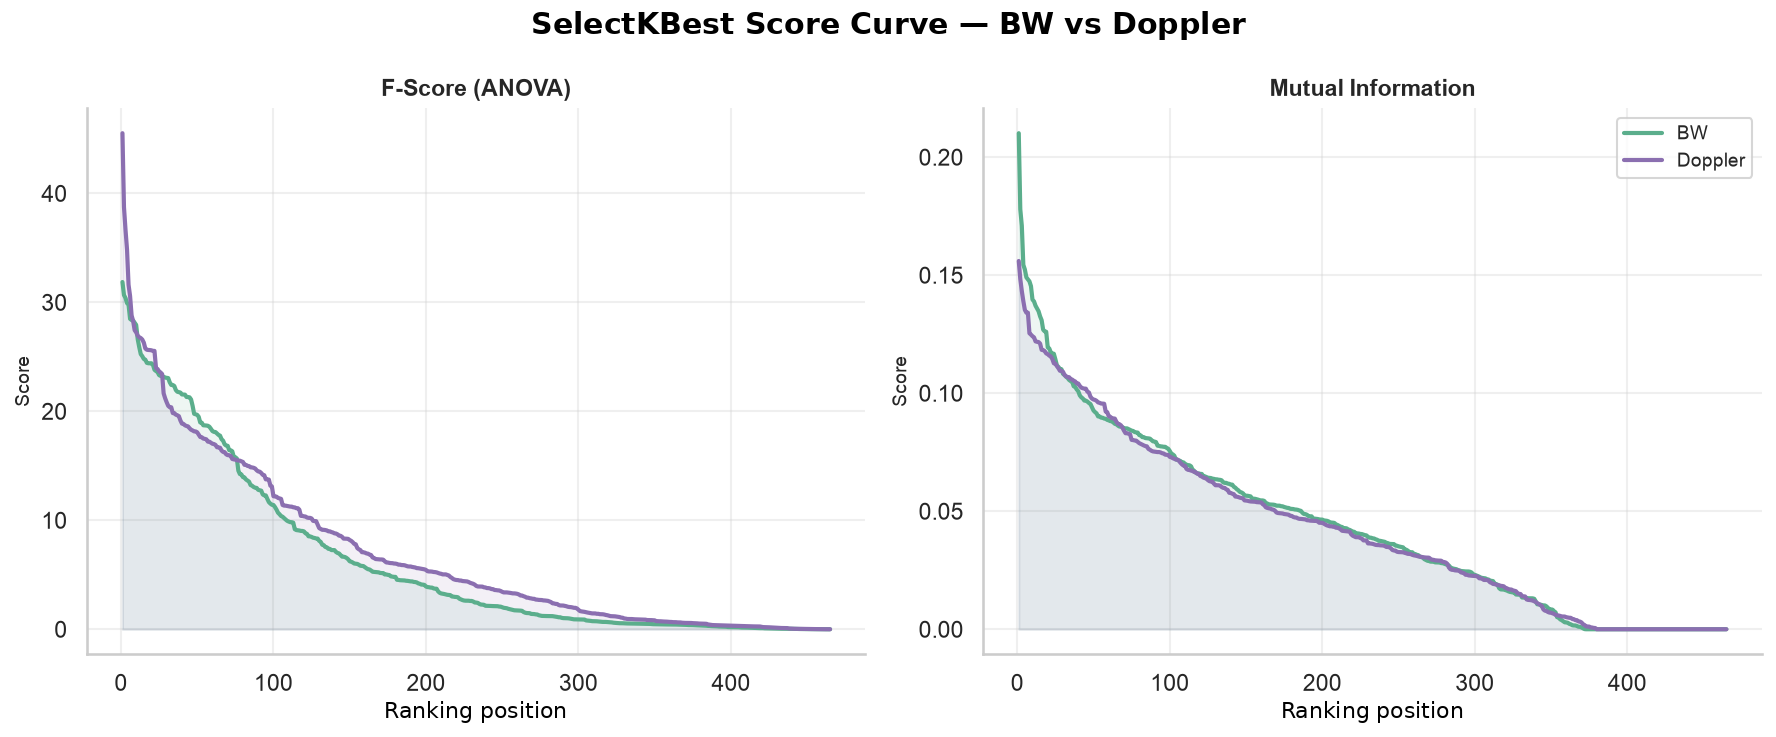
\includegraphics[width=0.9\textwidth]{Images/figure2_kbest_score_curve.png}
    \caption{Discriminative capacity curve for each statistical criterion. On the right, the feature ranking curve based on ANOVA; on the left, based on Mutual Information.}
    \label{fig:pieChart}
\end{figure}

In the Doppler dataset, the most discriminative feature according to the ANOVA F-score was "LL-gldm-DepEntropy" (F=45.52), with a score considerably higher than that observed in BW (F=31.86), suggesting that this modality has a more discriminative character than BW with respect to ANOVA. Mutual Information shows the inverted process: the most discriminative a feature is "LH-gldm-LDE" from the BW images, and the scores from this mode surpass all of the top 5 from the Doppler mode. 

\begin{table*}[h]
    \centering
    \caption{Top-5 most discriminative features per dataset, according to ANOVA F-score and Mutual Information}
    \label{tab:kbest-ranking}
    \resizebox{0.80\textwidth}{!}{%
    \begin{tabular}{c l r l r}
        \toprule
        \multirow{2}{*}{\textbf{Rank}} & \multicolumn{2}{c}{\textbf{ANOVA F-score}} & \multicolumn{2}{c}{\textbf{Mutual Information}} \\
        \cmidrule(lr){2-3} \cmidrule(lr){4-5}
         & \textbf{Feature} & \textbf{Score} & \textbf{Feature} & \textbf{Score} \\
        \midrule
        \multicolumn{5}{l}{\textit{Dataset: BW}} \\
        \midrule
        1 & LH\_glrlm\_GLNUN          & 31.86 & LH\_gldm\_LDE   & 0.210 \\
        2 & LH\_firstorder\_Entropy   & 30.67 & LH\_glrlm\_RP   & 0.178 \\
        3 & LH\_firstorder\_Unif.     & 30.40 & LH\_glszm\_LAHGLE & 0.171 \\
        4 & LH\_glcm\_SumEntropy      & 29.93 & LH\_glcm\_Idm   & 0.154 \\
        5 & LH\_glcm\_JointEntropy    & 29.77 & LH\_glcm\_Id    & 0.152 \\
        \midrule
        \multicolumn{5}{l}{\textit{Dataset: Doppler}} \\
        \midrule
        1 & LL\_gldm\_DepEntropy      & 45.52 & LH\_glrlm\_GLNUN  & 0.156 \\
        2 & LH\_glszm\_SAE            & 38.74 & HH\_gldm\_LDHGLE  & 0.148 \\
        3 & LH\_glszm\_SZNUN          & 36.66 & HH\_glcm\_MaxProb & 0.143 \\
        4 & HL\_glrlm\_RunEntropy     & 34.84 & LH\_gldm\_GLVar   & 0.139 \\
        5 & LL\_ngtdm\_Coarseness     & 31.61 & LL\_glcm\_Idmn    & 0.135 \\
        \midrule
    \end{tabular}}
    \vspace{4pt}

    \noindent\parbox{\textwidth}{\footnotesize \textbf{Note:} Abbreviations used in the table: GLNUN = GrayLevelNonUniformityNormalized; SZNUN = SizeZoneNonUniformityNormalized; LDE = LargeDependenceEmphasis; RP = RunPercentage; LAHGLE = LargeAreaHighGrayLevelEmphasis; SAE = SmallAreaEmphasis; LDHGLE = LargeDependenceHighGrayLevelEmphasis; GLVar = GrayLevelVariance; Unif. = Uniformity; DepEntropy = DependenceEntropy.}
\end{table*}

The graph in figure \ref{fig:pieChart} illustrates the behavior of the discriminative scores throughout the entire feature ranking, for the two criteria (F-score (ANOVA) and Mutual Information). The inversion of distinctive capacity between the BW and Doppler sets is also observed in the score curves by ranking position. Under the ANOVA F-score criterion, the highest value is obtained by the Doppler set's curve, while under the Mutual Information criterion, the BW set's curve shows the highest initial score.

Under both criteria, the discriminative potential is strongly concentrated in the first positions of the ranking. In all cases, an abrupt drop in score is observed already within the first few dozen features, followed by a long, progressively flatter tail, until stabilization near zero.


\subsection{Analysis of Machine Learning Models}

Tables \ref{tab:top5-cv-trilha-a} (Track A) and \ref{tab:top5-cv-trilha-b} (Track B) present the five classifiers with highest mean AUC obtained in cross-validation, along with respective standard deviation across folds

\begin{table}[h]
    \centering
    \begin{minipage}{0.48\textwidth}
        \centering
        \caption{Top 5 classifiers in cross-validation (Track A, exemplified for K=20)}
        \label{tab:top5-cv-trilha-a}
        \scriptsize
        \setlength{\tabcolsep}{3pt}
        \begin{tabular}{clc}
            \toprule
            \textbf{Dataset} & \textbf{Model} & \textbf{AUC} \\
            \midrule
            \multirow{5}{*}{BW}
                & 1. Coarse Gaussian SVM    & 0.779 $\pm$ 0.087 \\
                & 2. Boosted Trees          & 0.772 $\pm$ 0.083 \\
                & 3. RUSBoosted Trees       & 0.772 $\pm$ 0.083 \\
                & 4. Bagged Trees           & 0.772 $\pm$ 0.064 \\
                & 5. Subspace Discriminant  & 0.769 $\pm$ 0.063 \\
            \midrule
            \multirow{5}{*}{Doppler}
                & 1. Subspace Discriminant  & 0.825 $\pm$ 0.065 \\
                & 2. Coarse Gaussian SVM    & 0.823 $\pm$ 0.078 \\
                & 3. Linear SVM             & 0.820 $\pm$ 0.058 \\
                & 4. Cosine KNN             & 0.819 $\pm$ 0.057 \\
                & 5. Logistic Regression    & 0.818 $\pm$ 0.061 \\
            \midrule
            \multirow{5}{*}{BW+Dop.}
                & 1. Subspace Discriminant  & 0.808 $\pm$ 0.057 \\
                & 2. Coarse Gaussian SVM    & 0.804 $\pm$ 0.085 \\
                & 3. Bagged Trees           & 0.794 $\pm$ 0.066 \\
                & 4. Medium Gaussian SVM    & 0.794 $\pm$ 0.076 \\
                & 5. Boosted Trees          & 0.792 $\pm$ 0.041 \\
            \bottomrule
        \end{tabular}
    \end{minipage}
    \hfill
    \begin{minipage}{0.48\textwidth}
        \centering
        \caption{Top 5 classifiers in cross-validation (Track B)}
        \label{tab:top5-cv-trilha-b}
        \scriptsize
        \setlength{\tabcolsep}{3pt}
        \begin{tabular}{clc}
            \toprule
            \textbf{Dataset} & \textbf{Model} & \textbf{AUC} \\
            \midrule
            \multirow{5}{*}{BW}
                & 1. Medium Gaussian SVM    & 0.798 $\pm$ 0.062 \\
                & 2. Cubic SVM              & 0.767 $\pm$ 0.020 \\
                & 3. Cosine KNN             & 0.762 $\pm$ 0.056 \\
                & 4. Coarse Gaussian SVM    & 0.759 $\pm$ 0.084 \\
                & 5. Bagged Trees           & 0.752 $\pm$ 0.077 \\
            \midrule
            \multirow{5}{*}{Doppler}
                & 1. Medium Gaussian SVM    & 0.825 $\pm$ 0.049 \\
                & 2. Coarse KNN             & 0.815 $\pm$ 0.083 \\
                & 3. Weighted KNN           & 0.806 $\pm$ 0.063 \\
                & 4. Subspace KNN           & 0.796 $\pm$ 0.083 \\
                & 5. Coarse Gaussian SVM    & 0.792 $\pm$ 0.087 \\
            \midrule
            \multirow{5}{*}{BW+Dop.}
                & 1. Medium Gaussian SVM    & 0.815 $\pm$ 0.055 \\
                & 2. Weighted KNN           & 0.787 $\pm$ 0.071 \\
                & 3. Subspace KNN           & 0.784 $\pm$ 0.078 \\
                & 4. Medium KNN             & 0.776 $\pm$ 0.077 \\
                & 5. Coarse KNN             & 0.766 $\pm$ 0.074 \\
            \bottomrule
        \end{tabular}
    \end{minipage}
\end{table}

In all studied scenarios, the best classifier is an SVM with Gaussian kernel (Coarse or Medium Gaussian) or a Discriminant (Subspace/Linear). Furthermore, in track A tree-models based (Boosted/Bagged/RUSBoosted Trees) appears among top five, which not observed in track B. In Track B, the Gaussian SVM dominated across all three datasets (BW: $0.798 \pm 0.062$; Doppler: $0.825 \pm 0.049$; BW+Doppler: $0.815 \pm 0.055$) For Track A, the value of K=20 was selected for this analysis. The motivation for this selection is addressed in section 3.3. In this scenario, the classifier varies according to the dataset used: Coarse Gaussian SVM for BW ($0.779 \pm 0.087$), and Subspace Discriminant for Doppler  ($0.825 \pm 0.065$) and BW+Doppler ($0.808 \pm 0.057$). This suggests that, as the feature space is reduced, the performance of each model becomes more sensitive to the characteristics of each dataset.     

In both tracks, the Doppler dataset obtained the highest AUC values, suggesting a greater discriminative capacity in the features extracted from Doppler-type images.

\subsection{Sensitivity Analysis to Parameter K}

Figure \ref{fig:k-seep} presents, for each value of K, the AUC on the test set (left graph) and, in the right graph, the distribution of the mean stratified 5-fold cross-validation AUC across all evaluated classifiers, represented by boxplots. The median of this distribution remained notably stable throughout the entire range of K evaluated, with variation below 0.04 per dataset. Additionally, the inter-quartile range of the boxes (which reflects the performance dispersion among candidate models) remained consistent across the K values, indicating that the relative ordering of the classifiers is not sensitive to the number of selected features. Together, these two aspects suggest that k-fold does not constitute a sufficiently sensitive criterion for determining the optimal value of K.

\begin{figure}[h]
    \centering
    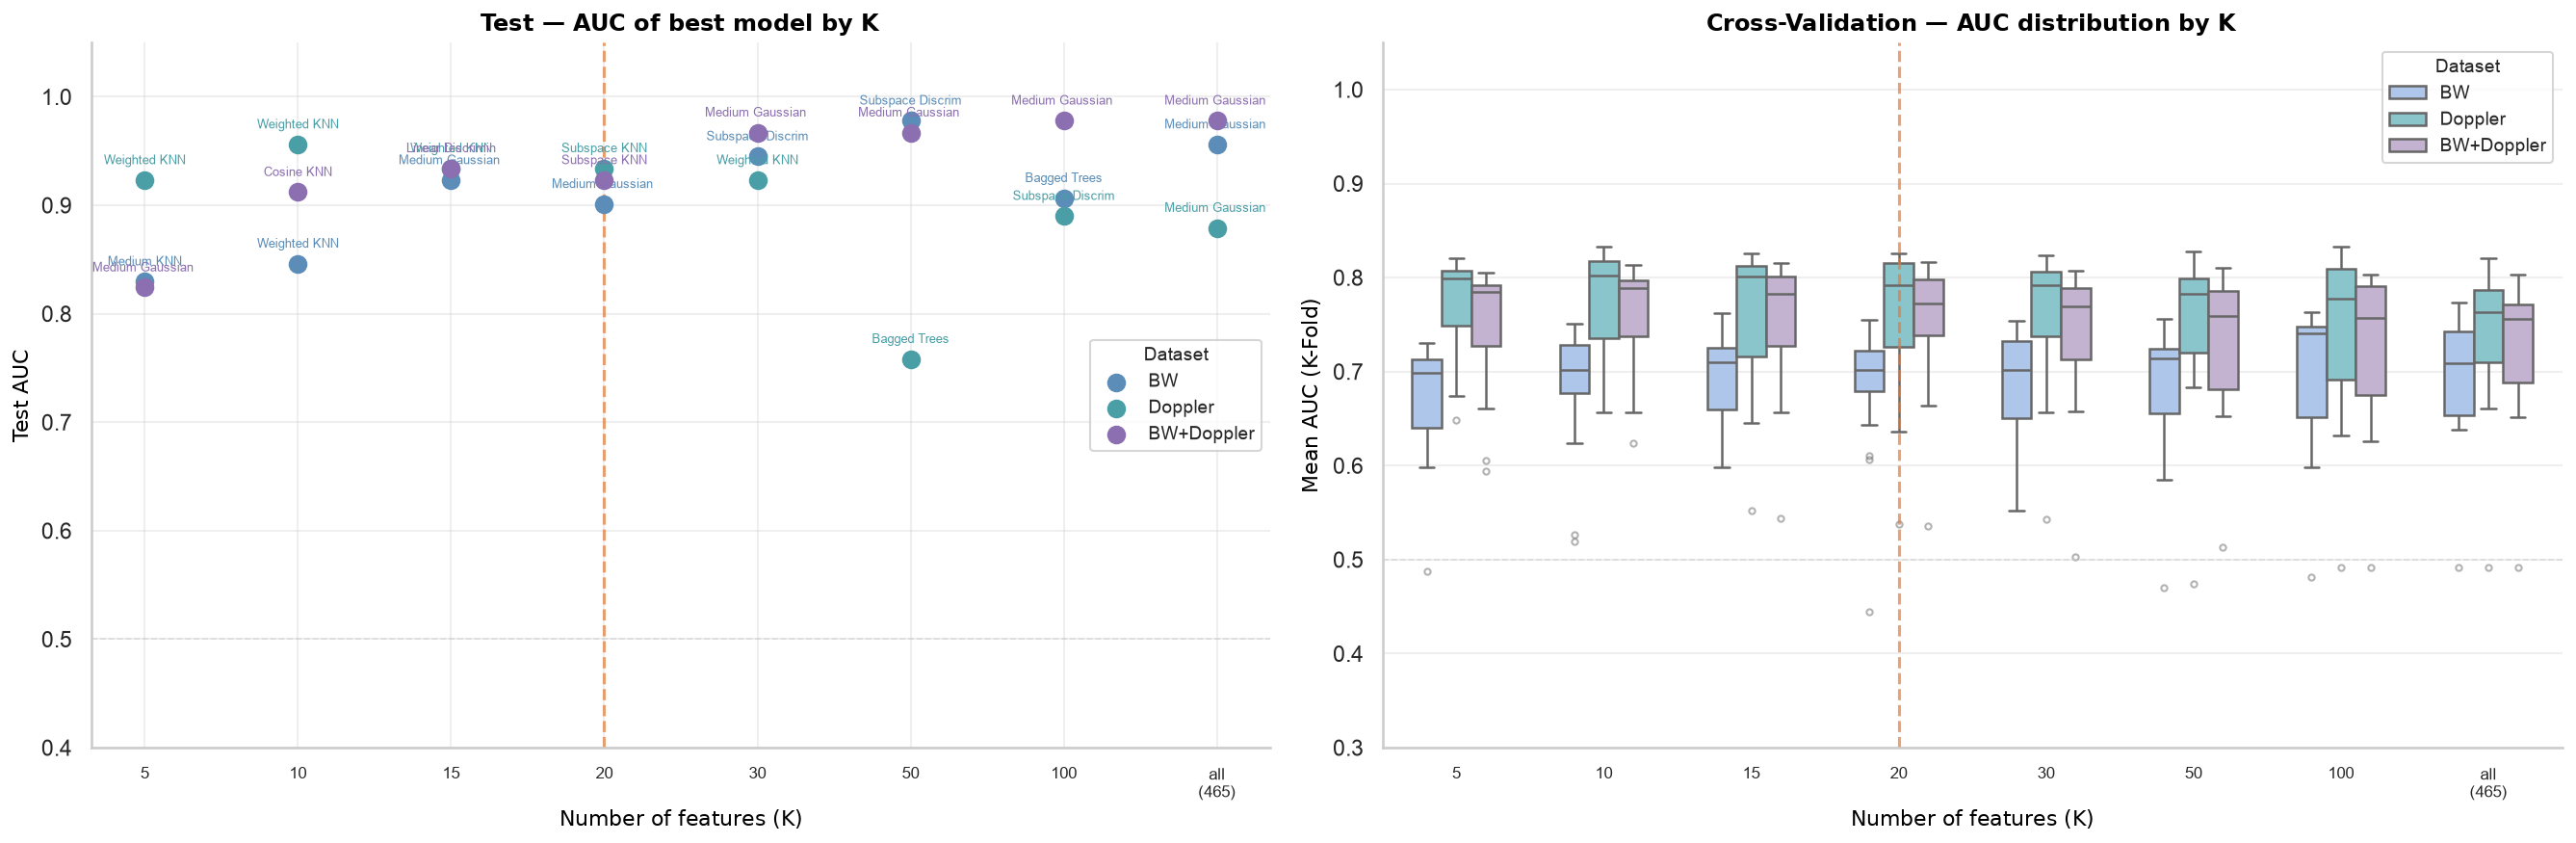
\includegraphics[width=0.9\textwidth]{Images/figure3_k_sweep_auc.png}
    \caption{AUC on the test set (left) and distribution of the mean AUC in k-fold cross-validation among
    all candidate classifiers, represented by \textit{boxplots}
    (right), for each value of K (number of features) evaluated.}
    \label{fig:k-seep}
\end{figure}


No monotonic trend was identified between the number of selected features and test performance. The Doppler dataset showed the highest sensitivity: at $K=50$ the AUC value was 0.758, which is considerably lower than the other points, which ranged from 0.879 to 0.956. The BW and BW+Doppler datasets exhibited more stable behavior.

\begin{table*}[h]
    \centering
    \caption{Performance of the best classifiers per dataset (on the test data) — Tracks A and B}
    \label{tab:resultados-youden}
    \resizebox{\textwidth}{!}{%
    \begin{tabular}{clcccccc}
        \toprule
        \textbf{Track} & \textbf{Dataset} & \textbf{Model} & \textbf{Sensitivity} & \textbf{Specificity} & \textbf{F1-Score} & \textbf{Accuracy} & \textbf{AUC} \\
        \midrule
        \multirow{3}{*}{A} & BW           & Coarse Gaussian SVM   & 0.714 & 1.000 & 0.833 & 0.900 & 0.868 \\
                            & Doppler      & Subspace Discriminant & 1.000 & 0.692 & 0.778 & 0.900 & 0.989 \\
                            & BW+Doppler   & Subspace Discriminant & 0.714 & 0.846 & 0.714 & 0.900 & 0.956 \\
        \midrule
        \multirow{3}{*}{B} & BW           & Medium Gaussian SVM   & 0.714 & 0.923 & 0.769 & 0.850 & 0.956 \\
                            & Doppler      & Medium Gaussian SVM   & 0.571 & 1.000 & 0.727 & 0.850 & 0.879 \\
                            & BW+Doppler   & Medium Gaussian SVM   & 1.000 & 0.923 & 0.933 & 0.950 & 0.978 \\
        \bottomrule
    \end{tabular}}
\end{table*}


At K=20, the results were: AUC=0.901, AUC=0.934, and AUC=0.923 (for BW, Doppler, and BW+Doppler, respectively). These values are close to the maximum values observed in the test set (0.978 for BW at K=50; 0.956 for Doppler at K=10; 0.978 for BW+Doppler at K=100), without the increase in dimensionality associated with higher values of K. It is worth noting that K=20 was fixed prior to the evaluation on the test set, preserving the validity of the comparison with Track B.

\begin{figure}[h]
    \centering
    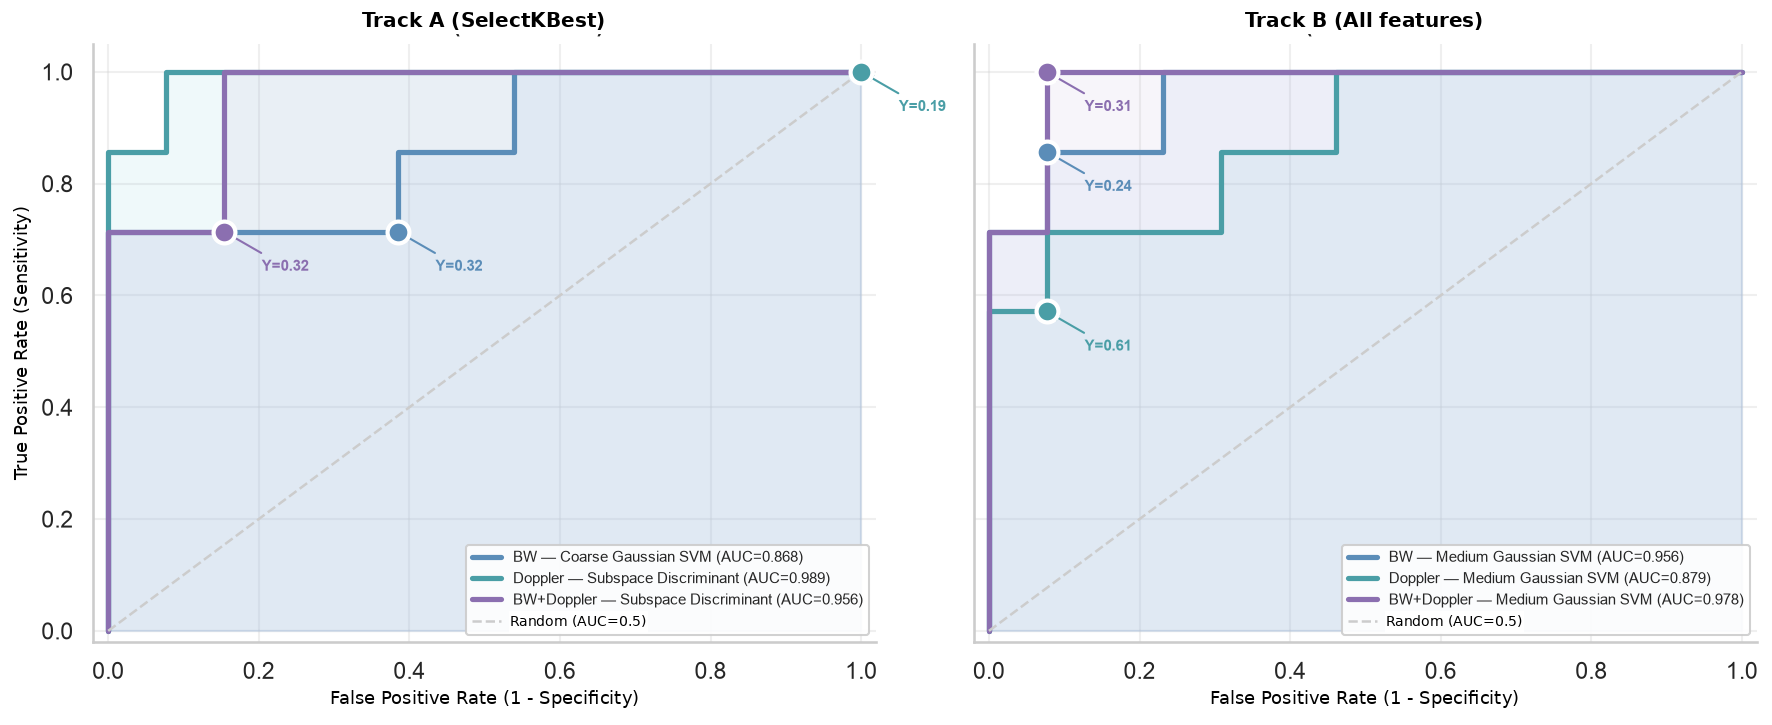
\includegraphics[width=0.9\textwidth]{Images/figure4_roc_curves.png}
    \caption{ROC curves on the test set with Track A (K=20 features) vs Track B (all features). Points mark the Youden threshold.}
    \label{fig:curva_roc}
\end{figure}

\subsection{Test Set Evaluation}

Table \ref{tab:resultados-youden} shows the evaluation results of the models on the test data for Track A and Track B, and figure \ref{fig:curva_roc} shows the ROC curve of the models from these tracks, after being trained with the entire dataset.

\begin{figure}[h]
    \centering
    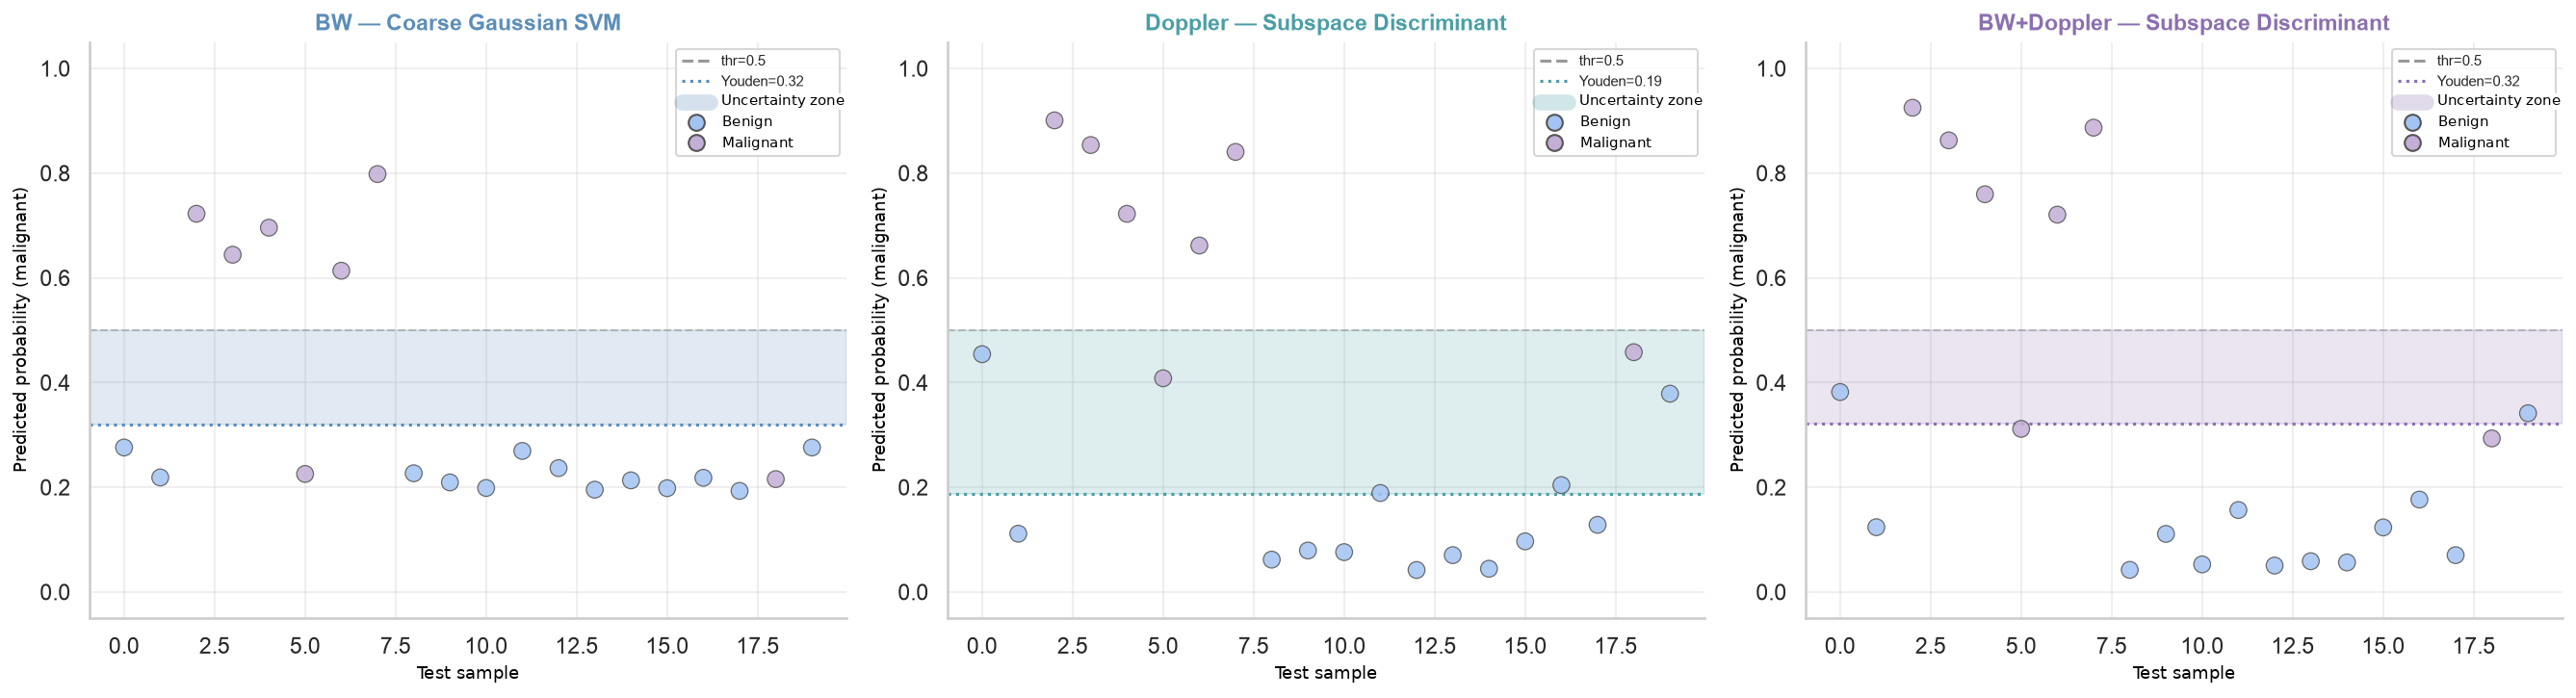
\includegraphics[width=1\textwidth]{Images/figure5_prob_distribution_trackA.png}
    \caption{Distribution of predicted probabilities for the test set samples (Track A). Horizontal lines indicate the 0.5 and Youden decision thresholds; point color denotes the true class of each lesion (purple = malignant, blue = benign).}
    \label{fig:predict_probs_a}
\end{figure}

\begin{figure}[h]
    \centering
    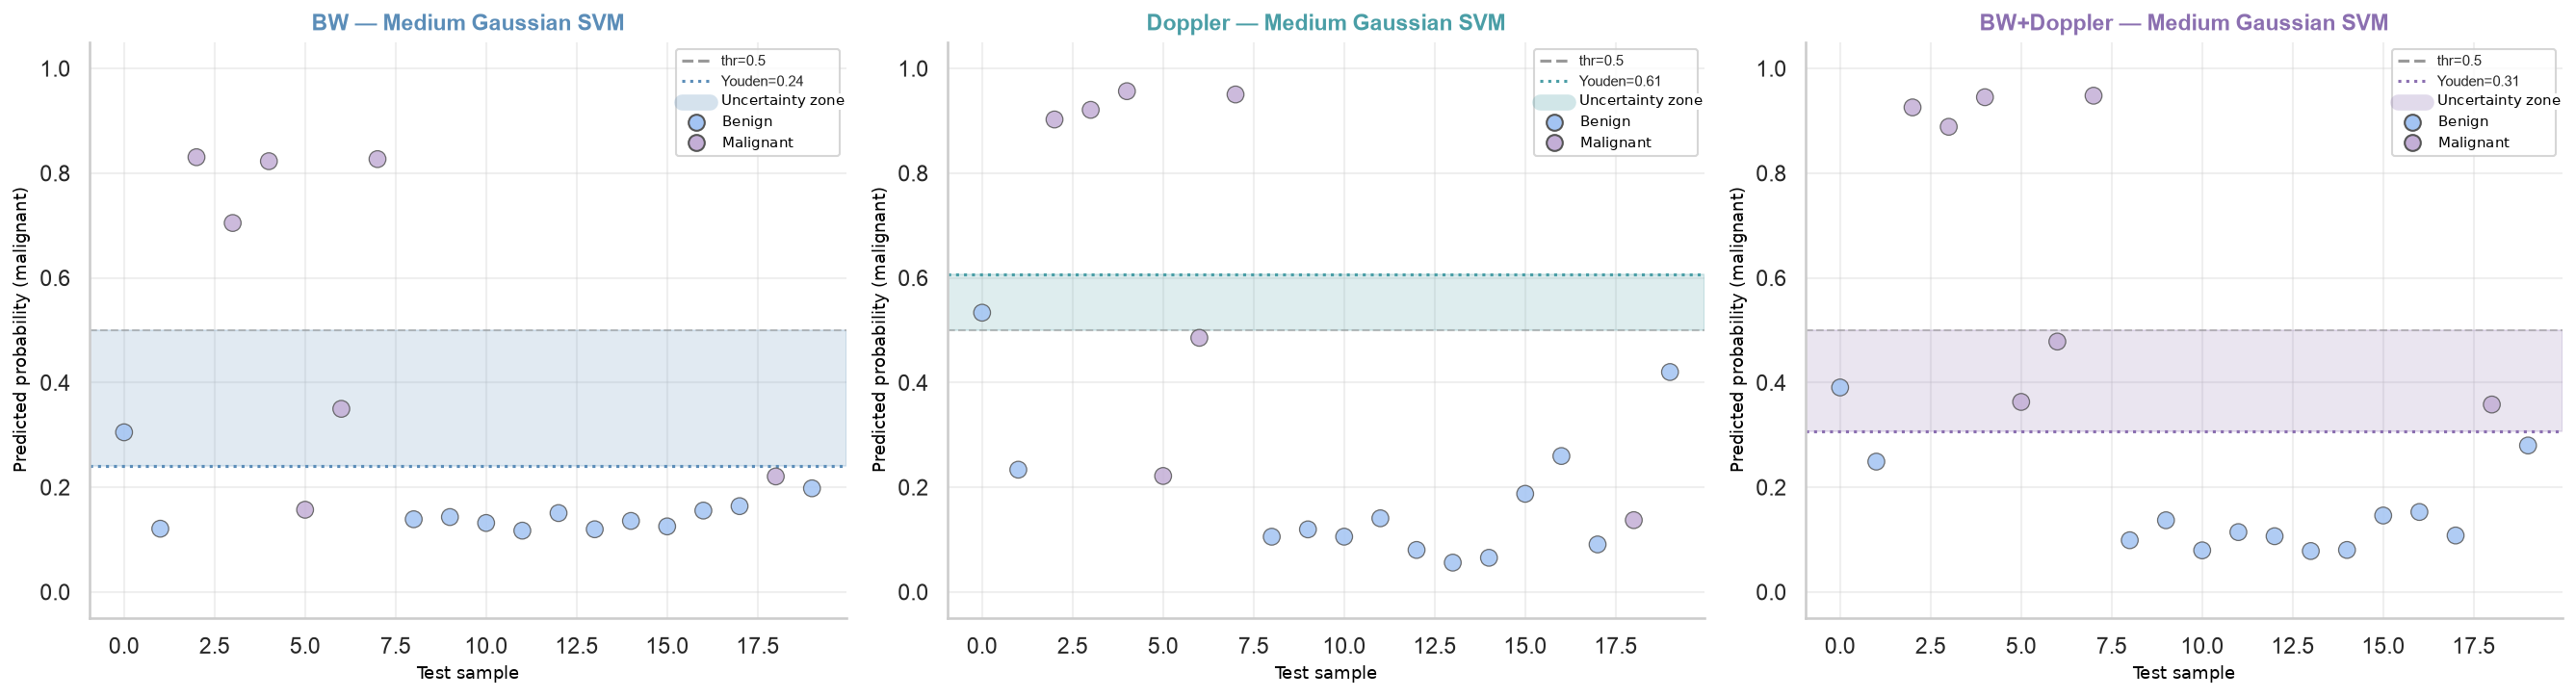
\includegraphics[width=1\textwidth]{Images/figure6_prob_distribution_trackB.png}
    \caption{Distribution of predicted probabilities for the test set samples (Track B). Horizontal lines indicate the 0.5 and Youden decision thresholds; point color denotes the true class of each lesion (purple = malignant, blue = benign).}
    \label{fig:predict_probs_b}
\end{figure}

The AUC was systematically higher than in cross-validation in almost all cases (e.g.: Doppler-A goes from 0.825 to 0.989; BW+Doppler-A from 0.808 to 0.956), which is expected given the small test set (n=20). Furthermore, in cross-validation, Track A obtained similar or slightly better performance (Doppler 0.825 equal; BW+Doppler 0.808 vs 0.815), however in the test set, Track B outperforms in BW (0.956 vs 0.868) and BW+Doppler (0.978 vs 0.956), while in Track A, Doppler wins (0.989 vs 0.879).

Graphs \ref{fig:predict_probs_a} and \ref{fig:predict_probs_b} show, respectively, the dispersion of predicted probability of the test data in Track A and Track B. Points above the threshold lines (0.5 and Youden) are classified as malignant, while points below are classified as benign. The color of each point indicates the actual class of the lesion: purple for malignant and blue for benign. In general, most benign samples are concentrated in the lower range of predicted probability (0.05 - 0.20), while malignant samples appear in the upper probability range (0.70-0.95). The region between the Youden threshold and 0.5 (uncertainty zone in graphs \ref{fig:predict_probs_a} and \ref{fig:predict_probs_b}), on the other hand, appears sparsely populated.

One benign sample (the first, index 0) receives abnormally high scores for a benign case: in Doppler-A (0.45), BW+Doppler-A (0.39), BW-B (0.31), and especially Doppler-B (0.53, even surpassing the 0.5 threshold)

\section{Discussion}

As reported in the work of Silva et al. (2026), their best model, trained on the same dataset and the same classification task as this work, the HFUS-Doppler, achieved an accuracy of $95.0\%$, a specificity of $100\%$, sensitivity of $85.7\%$, F1-Score of $92.3\%$ and AUC of 0.98 \cite{daSilva2026}. In contrasts, the best model proposed in the present work, a Gaussian SVM with the BW+Doppler dataset from Track B, ties or exceeds in nearly all metrics, achieved an accuracy of  $95.0\%$, AUC of 0,978, sensitivity of $100\%$ an specificity of $92.3\%$. These results also expressively surpass the EfficientNet B4 model reported by Laverde-Saad et al (2022). (original work that made dataset used available), whose best result on the test dataset was $77.1\%$ of accuracy, $73.3\%$ of sensitivity  and $80.0\%$ of specificity \cite{LaverdeSaad2021}. The classifier's performance compared to a deep neural network trained directly on image pixels suggests that the textural and morphological information captured by radiomics is sufficient to match dedicated CNNs in discriminative capacity, with the advantage of maintaining greater model interpretability.

The main difference between the model in this work and the HFUS-Doppler proposed by Silva et al. (2026) lies in the trade-off between specificity and sensitivity. While the CNN model achieved $100\%$ specificity, the SVM reverses this pattern, reaching $100\%$ sensitivity. In clinical contexts, sensitivity is considered a priority metric, since a false positive only leads to additional investigation, whereas a false negative (a malignant lesion classified as benign) can delay diagnosis and the start of treatment. In this sense, although both models show comparable overall performance, the model proposed in this work is more aligned with the desired behavior in a diagnostic screening scenario.

The visual analysis of the predicted probability plots in figures \ref{fig:predict_probs_a} and \ref{fig:predict_probs_b} helps to further clarify this difference. In the work of Silva et al. (2026), the HFUS-Doppler model yields predictions with widely spread probabilities, with samples close to the Youden threshold, which the authors refer to as a gray zone. In our BW+Doppler-B model, most malignant samples were above 0.5, and most benign samples below 0.15, far from this zone and from the Youden threshold (J = 0.307), indicating a stronger signal of discriminative confidence from the model than from the CNN. This supports the assumption that texture and morphology information from radiomic features alone is sufficient to model the proposed classification task, without the need to resort to the complexity of convolutional networks.

In the range between the Youden threshold and the 0.5 threshold, it is clearly possible to define a region. in the present work refers to it as the model’s uncertainty region, meaning that samples falling within this range exhibit ambiguous predictions, in which the model does not reach sufficient confidence for a definitive classification in either direction.

Artificial intelligence models have been extensively explored in the current scenario; however, the majority of studies using this imaging modality focus on the study of deep learning architectures \cite{Qin2025}. But training and performing inference with these requires specialized computational infrastructure, mainly high-performance GPUs \cite{Czajkowska2021-2}. In contrast, the approach of basic classifiers and radiomic features used in in the present work does not require such robust computational resources, eliminating the need for GPUs. Once the features are extracted, the models are trained in seconds, making the pipeline reproducible on conventional hardware. 

Despite the significant reduction in computational cost, the best-performing model (Medium Gaussian SVM, BW+Doppler) was trained in approximately 51 ms on an Intel Core i5-7267U processor with 8 GB of RAM, without GPU usage, and the results obtained remain competitive, matching or surpassing deep learning approaches using the same dataset reported in the literature \cite{LaverdeSaad2021, daSilva2026}. Models with a smaller number of parameters tend to generalize better and are less prone to overfitting in scenarios with limited data. This way, the radiomic approach proves suitable for the HFUS context, which shares in the data scarcity issue, reducing the barrier to entry in the clinical setting.

Table \ref{tab:resultados-youden} shows that in both Track A and Track B, the best-performing models were those using the combined data (BW+Doppler). Furthermore, in Track A, the Subspace Discriminant model, trained with only 20 features and using only Doppler images, outperformed in AUC (AUC=0.989) the models trained with only BW in Track A (AUC=0.868) and Track B (AUC=0.956). These results can be explained by the important role of Doppler images in providing information (vascular and hemodynamic data of the individual) that is essential for the comprehensive assessment of differences between dermal lesions, as described in the DERMUS guideline \cite{Wortsman2016}.

The literature reinforces this argument. Qin et al. (2025), one of the few works addressing the extraction of radiomic features for lesion classification, reported an AUC of 0.914 for their best model, a multilayer perceptron (MLP) network using only BW-mode images \cite{Qin2025}. The best model in the present study, trained with the combination of both image types, outperformed this one in AUC. Faita et al. (2021) also demonstrated that $85\%$ of malignant melanomas acquired intralesional vascularization, compared to only $26\%$ of melanocytic nevi \cite{Faita2022}. This indicates that patterns captured in Doppler constitute highly discriminative markers between lesion classes.

However, the difference between the cross-validation results and the test set results reveals a weakness related to the reduced number of samples. The test set had only 20 images (13 malignant and 7 benign), which makes the test set intrinsically unstable. A small variation in the composition of the test set samples can alter the results. Notably, the AUC was higher on the test data in all cases. This does not represent a greater generalization capacity, but rather sample variation between cross-validation and the test set. Thus, the results in this work should be interpreted as preliminary evidence of these models' performance and of the need for larger datasets to confirm the robustness of the method.

In summary, the experimental results highlight the advantages of training classical models with radiomic features to classify cutaneous lesions. Despite their simple architecture, the models remain competitive, obtaining results comparable to those in the literature. The low computational and data cost represents an advantage in clinical contexts where training resources are limited. However, the limited amount of publicly available HFUS data represents a weakness of the study. Future research should focus on expanding the dataset, validating the proposed models on larger samples from different centers. Even so, the approach proves promising as a low-cost, more interpretable alternative to deep learning in the diagnosis of cutaneous lesions in HFUS.

\printbibliography

% \section*{Acknowledgments}
% This study was financed in part by the Coordenação de Aperfeiçoamento de Pessoal de Nível Superior - Brasil (CAPES) - Finance Code 001


\end{document}